%\documentclass[a4paper,oneside,onecolumn]{article}
\documentclass[journal=nalefd,manuscript=letter]{achemso}
\setkeys{acs}{articletitle=true}
\usepackage{graphicx}
\usepackage{amsmath}
\usepackage{amssymb}
\usepackage{subfigure}
\usepackage{xr}
%%% This is for adding a footer with the time of the compilation of the file.
%%% Useful for versioning of printed copies.
%\usepackage{datetime}
%\usepackage{fancyhdr}
%\fancyfoot[L]{\fontsize{8}{12} \selectfont \today $\,$ \currenttime}
%\pagestyle{fancy}
%%%%%%%%%%%%%%%%%%%%%%%%%%%%%%%%%%%%%%%%%%%%%%%%%%%%%%%%%%%%%%%%%%%%%
%%%%%%%%%%%%%%%%%%%%%%%%%%%%%%%%%%%%%%%%%%%%%%%%%%%%%%%%%%%%%%%%%%%%%

\usepackage[version=3]{mhchem} % Formula subscripts using \ce{}
\usepackage[T1]{fontenc}       % Use modern font encodings
\renewcommand{\thefigure}{S\arabic{figure}}

\newcommand{\nm}{\ensuremath{\,\textrm{nm}}}
\newcommand{\um}{\ensuremath{\,\mu\textrm{m}}}
\newcommand{\eV}{\ensuremath{\,\textrm{eV}}}
\newcommand{\uM}{\ensuremath{\,\mu\textrm{M}}}
\newcommand{\uW}{\ensuremath{\,\mu\textrm{W}}}
\newcommand{\pM}{\ensuremath{\,\textrm{pM}}}
\newcommand{\meV}{\ensuremath{\,\textrm{meV}}}
\newcommand{\pwr}{\ensuremath{\,\textrm{kW/cm}^2}}
\newcommand{\CPS}{\ensuremath{\,\textrm{CPS}}}
\newcommand{\kCPS}{\ensuremath{\,\textrm{kCPS}}}
\newcommand{\atto}{\ensuremath{\textrm{Atto}\,647\textrm{N}}}

\author{A. Carattino}
\author{V.I.P. Keizer}
\author{M.J.M Schaaf}
\author{M. Orrit}

\title{Background suppression in imaging gold nanorods through detection of anti-Stokes emission}

\keywords{Gold nanorods, Plasmon, Imaging, Anti-Stokes, Bio-imaging, Confocal}

\begin{document}
\maketitle

\section{Setup}

\begin{figure}[htp]
 \centering
 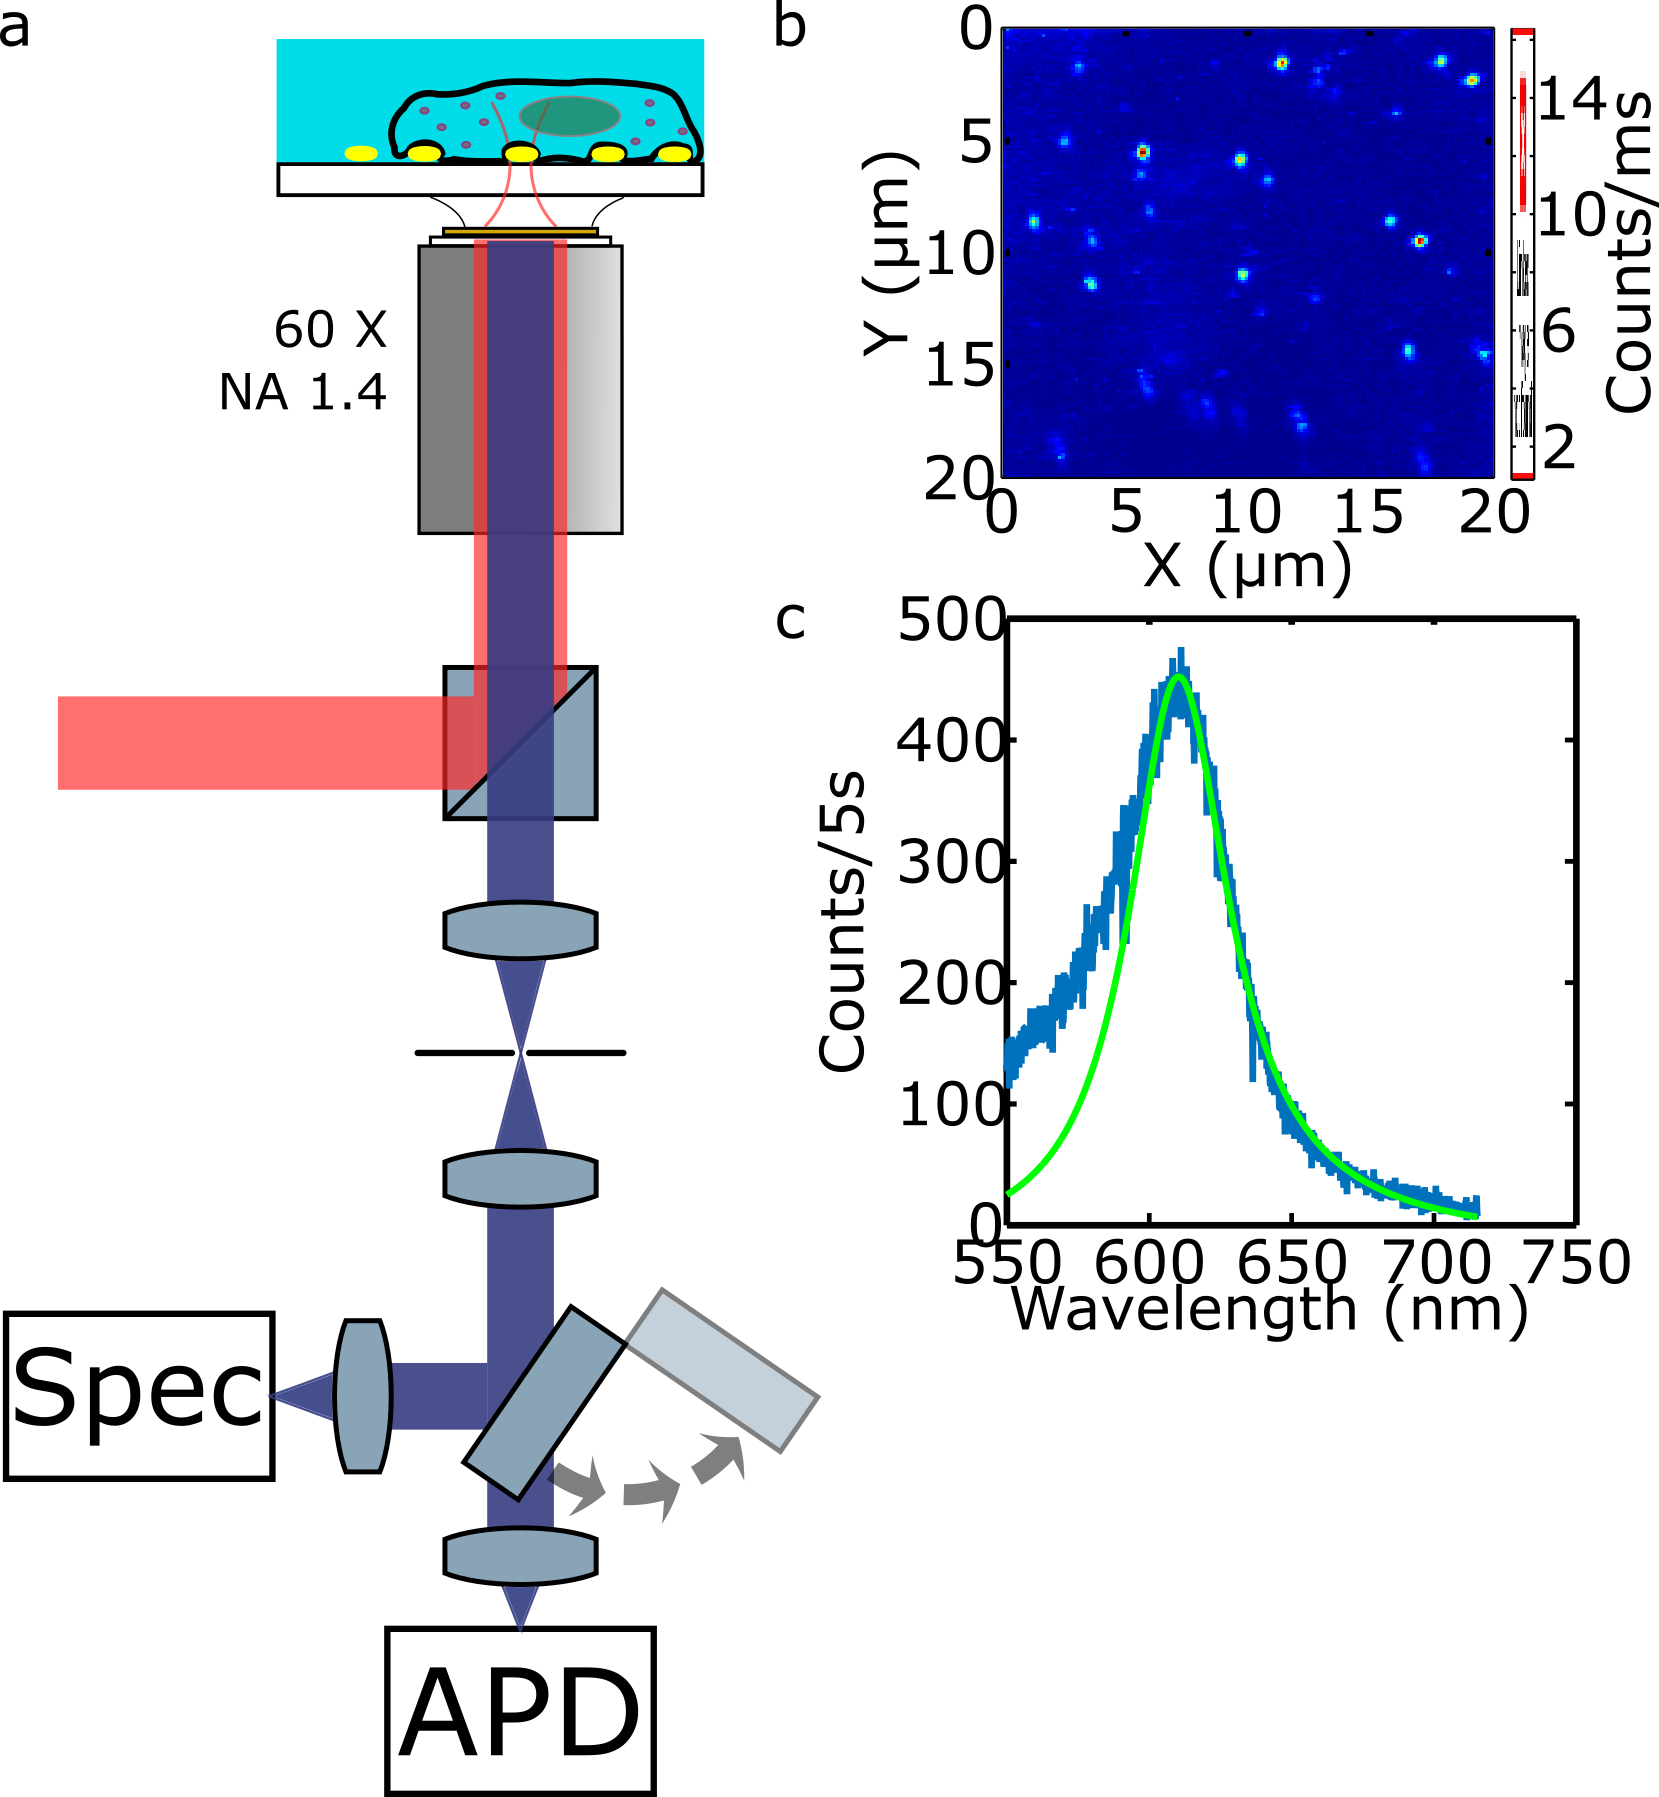
\includegraphics[width=0.45\textwidth]{Figures/Supplementary/01_Setup/setup_1.png}
 \caption{Experimental setup and examples of observations. a) Simplified
 schematic of the confocal microscope employed during the measurements. b) A
 typical 1-photon luminescence raster scan of the sample immersed in water c)
 luminescence spectrum of a single rod.}
 \label{fig:setup}
\end{figure}

Figure \ref{fig:setup} shows the schematic of the confocal microscope employed
in the experiments. It is important to note the presence of a $50/50$
beamsplitter before the objective. Exchanging it for an appropriate dichroic
mirror would increase the collection efficiency. In this work we chose not to do
it because the beamsplitter allows to collect both the full emission under
$532\nm$ excitation and the Stokes/anti-Stokes emission under $633\nm$ without
changes in the optical path. 

\section{Uv-Vis spectrum}

\begin{figure}[htp]
 \centering
 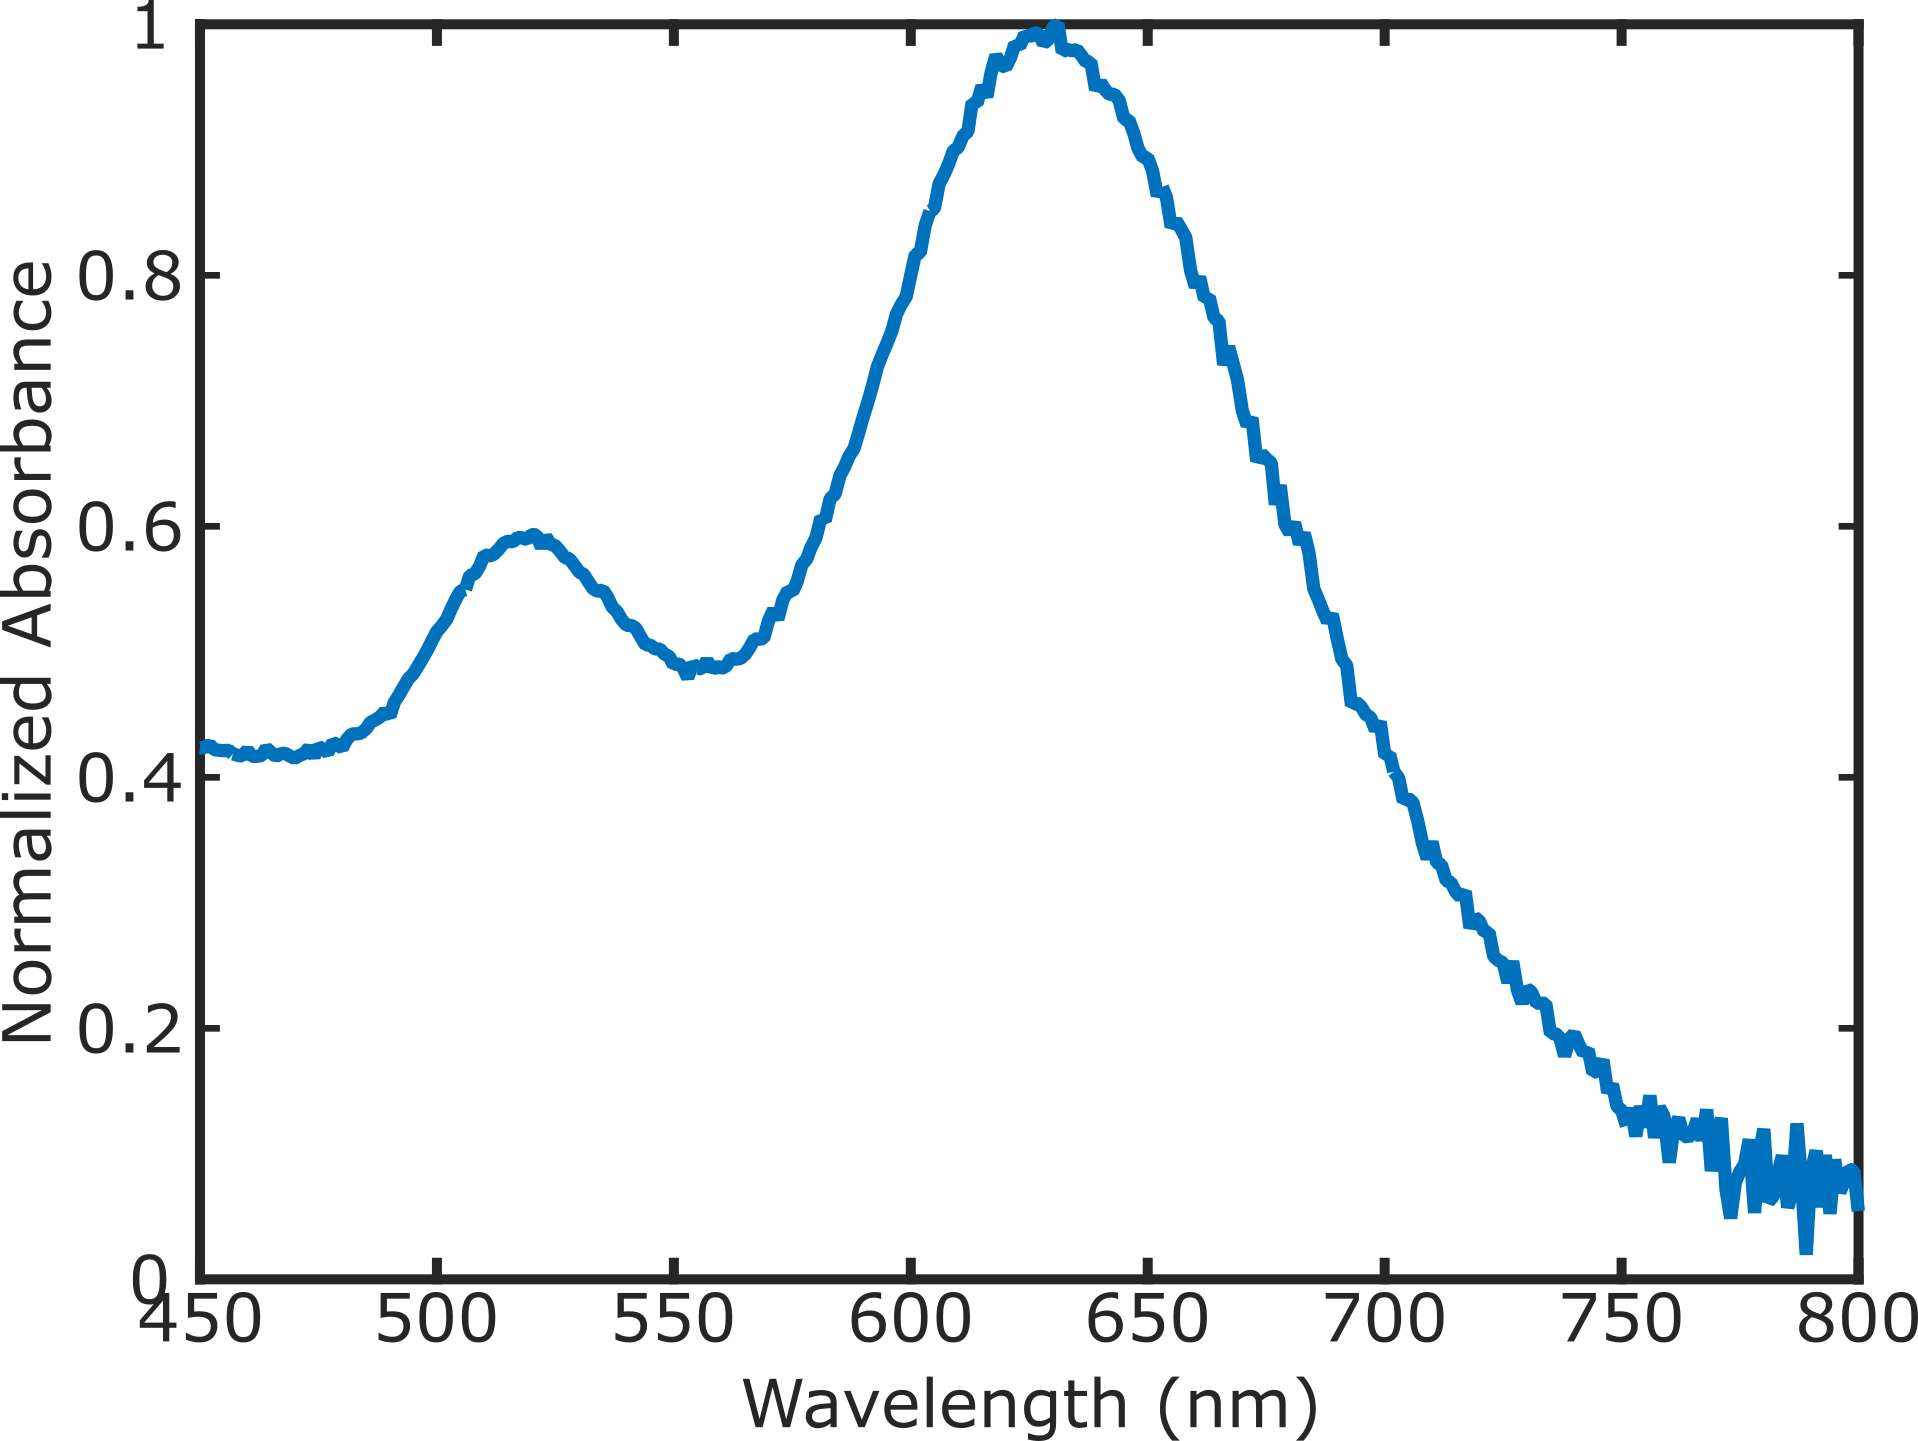
\includegraphics[width=0.45\textwidth]{Figures/Supplementary/02_UV-Vis/uvvis.png}
 \caption{Normalized extinction spectrum of a suspension of nanorods after
 synthesis. The resonance maximum is located at $630\nm$.}
 \label{fig:uvvis}
 \end{figure}
 
 Figure \ref{fig:uvvis} shows the extinction spectrum of the nanorod samples
 used throughout this work. Two peaks are clearly distinguishable, one around
 $630\nm$ that corresponds to the longitudinal plasmon resonance (LPR) of
 particles with sizes $50\nm\times23\nm$ and a second one at around $520\nm$.
 This peak also includes contributions of spheres as by-products of the
 synthesis of the rods. The transverse plasmon resonance is also located at the
 same wavelength but is much weaker than the LPR. In a sample consisting exclusively of rods, the transverse resonance would be barely observable in a UV-Vis
 spectrometer.
 
 \section{Filters}

\begin{figure}[htp]
 \centering
 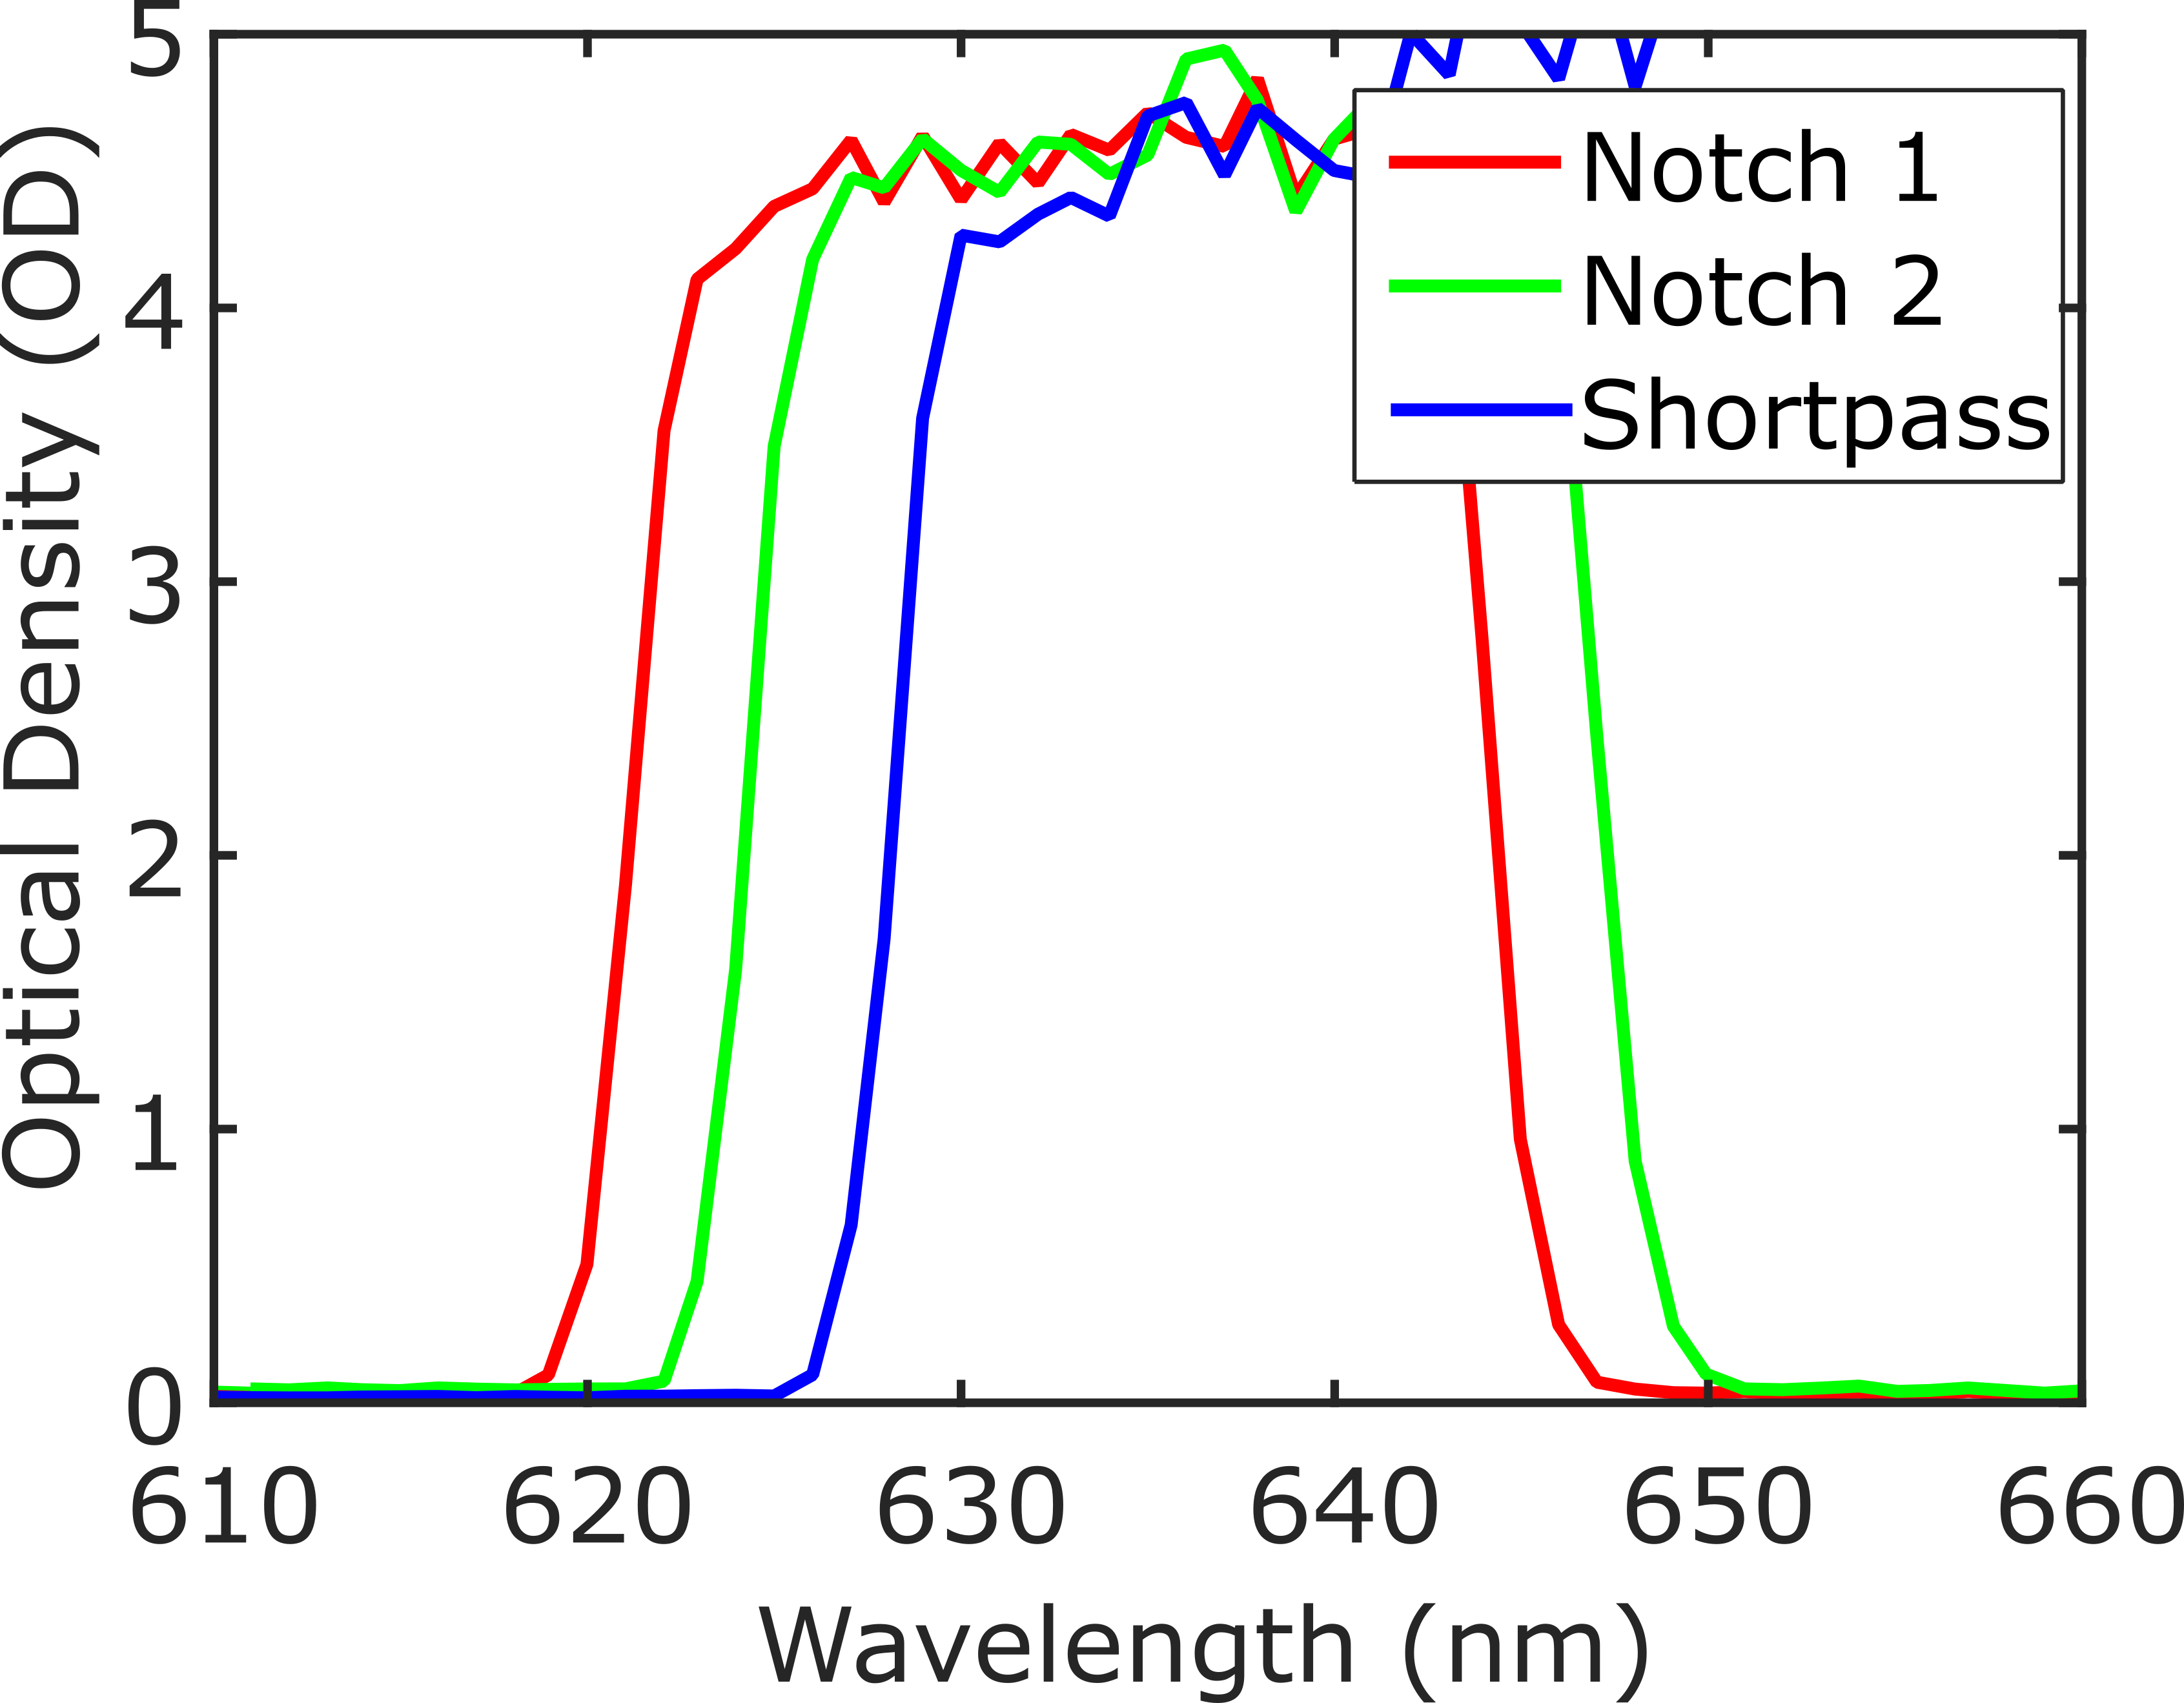
\includegraphics[width=0.45\textwidth]{Figures/Supplementary/03_Filters/filters.png}
 \caption{Transmission spectrum of two notch filters and a short pass
 filter (Semrock).}
 \label{fig:filters}
 \end{figure}
 
The selection of filters plays a crucial role in the signal acquired. Since the
main part of the anti-Stokes emission is concentrated around the excitation
wavelength, it is important to select filters that have a high transmission
close to the laser line. Figure \ref{fig:filters} shows the normalized
absorption spectrum of two notch filters and a short pass. Both notch filters are
branded as $\textrm{NF}03-633\textrm{E}-25$ but show a slightly different
absorption spectrum, shifted roughly $4\nm$ from each other. The shortpass
filter (branded as $\textrm{SP}01-633\textrm{RU}-25$) shows the transition to
transmission even closer to the laser line. 

For many fluorescence applications the exact shape of the transmission
spectrum of the filters does not play a crucial role. However for anti-Stokes
imaging, since the shape of the emission is exponential-like, minute
changes in the transmission spectrum can have a great impact on the signal collected. For example, changing from
a detection path with a spectrum like notch $1$ to one like shortpass (i.e.
shifting in about $7\nm$ the edge of the filter) increases the collected number
of photons by about $50\%$. 

In this work, since only one filter does not provide enough attenuation, care was
taken to always employ the notch with the most favorable transmission spectrum
in combination with either a shortpass or a longpass filter. Ideally, two
shortpass filters would have been the best solution.
 
 \section{TEM Images of rods}
 
\begin{figure}[htp]
 \centering
 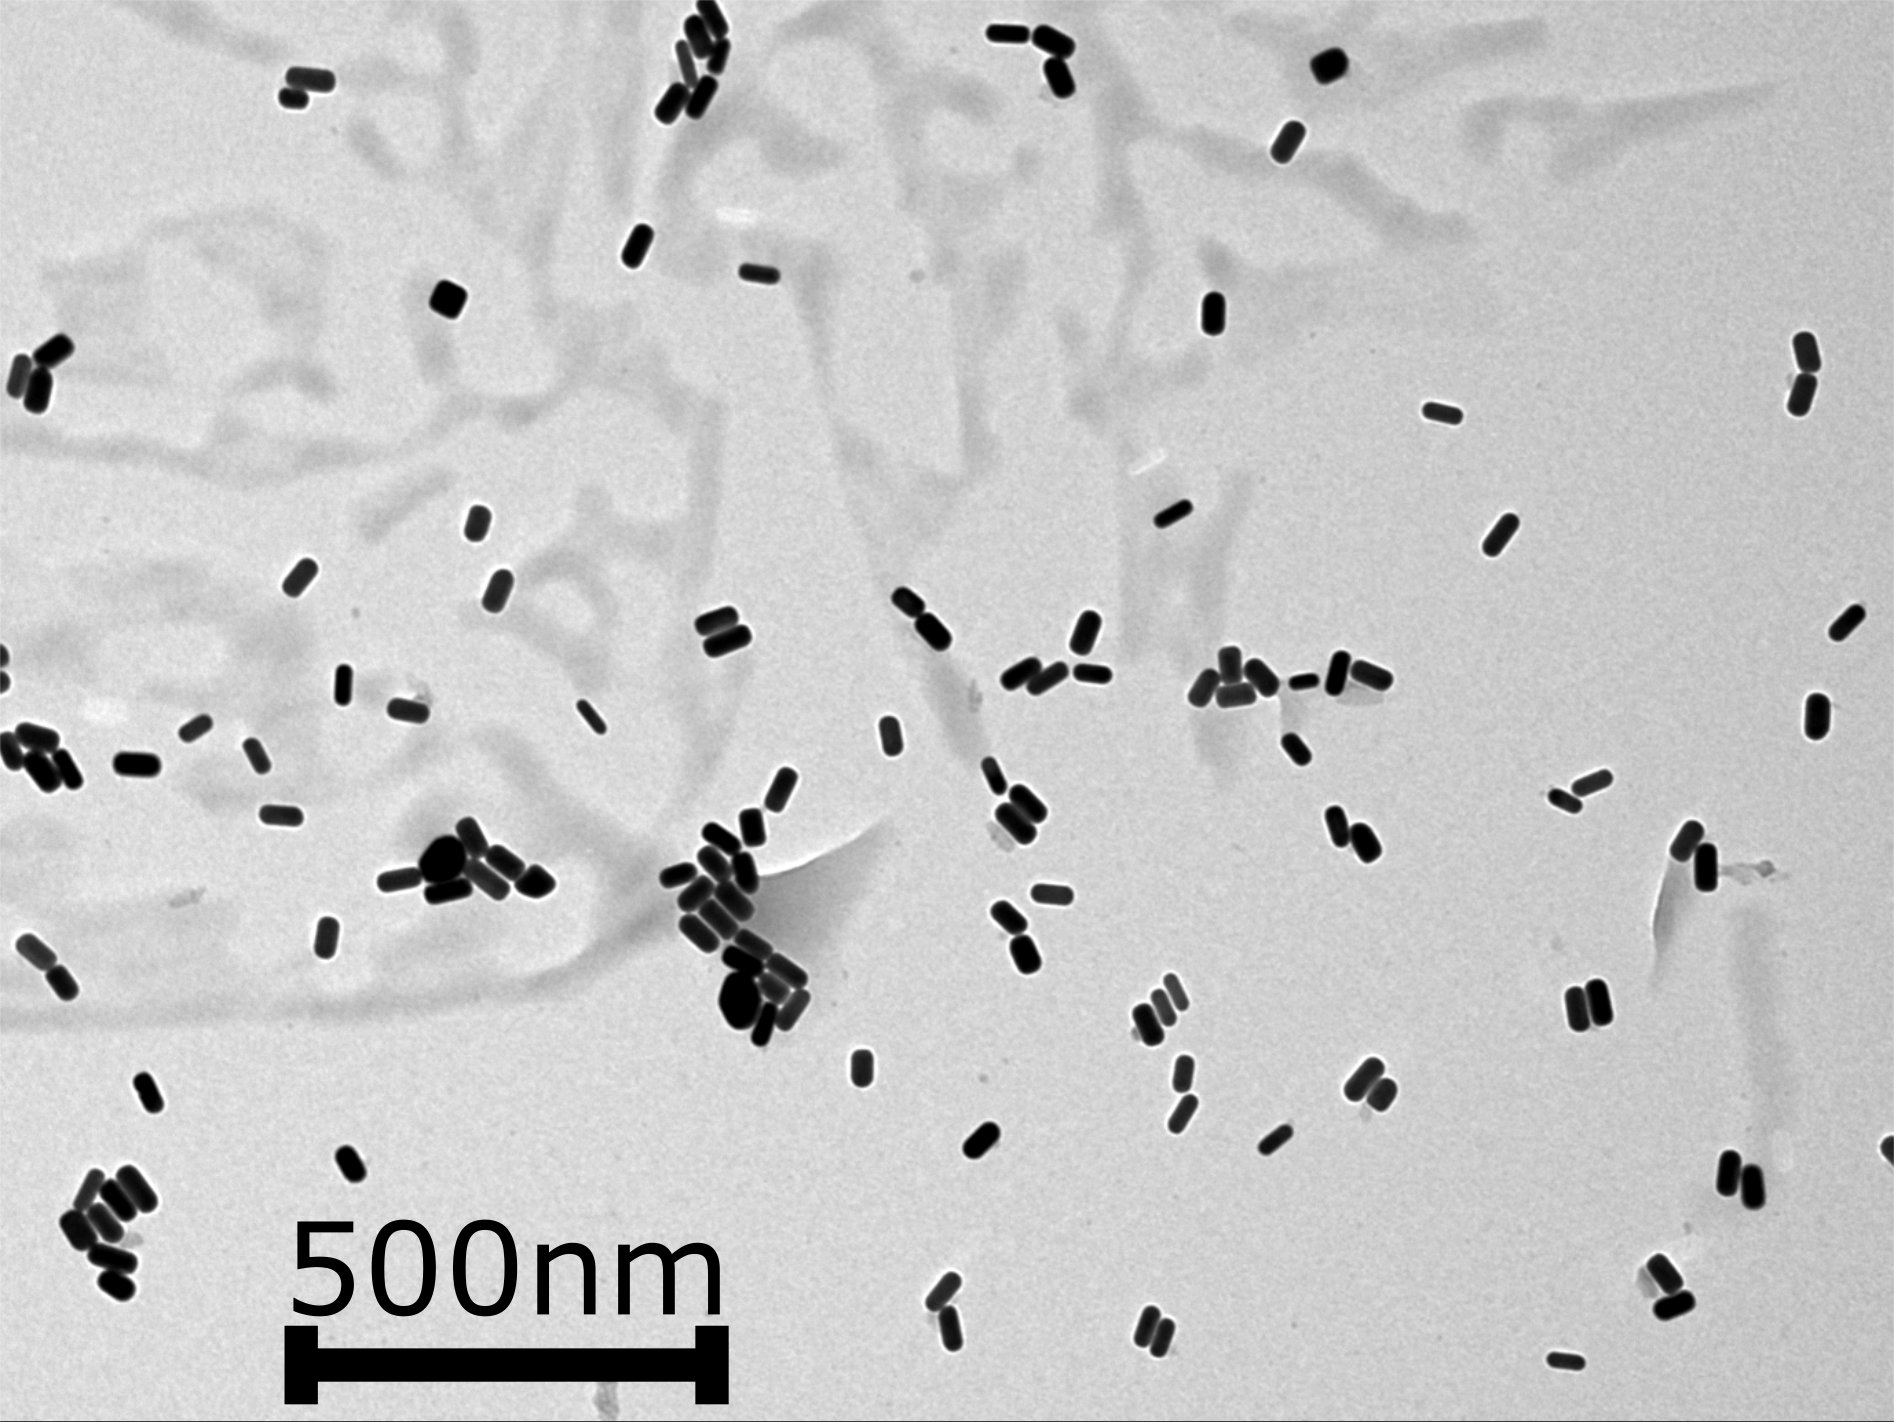
\includegraphics[width=0.45\textwidth]{Figures/Supplementary/04_TEM/tem.png}
 \caption{TEM image of the nanorod sample. The scale bar is $500\um$. }
 \label{fig:TEM}
 \end{figure}
 
Figure \ref{fig:TEM} shows an example TEM image of the gold nanorod sample.
Analysis on the dimensions of the particles yield an average length of $50\nm$
and diameter of $23\nm$. This is consistent with the plasmon observed in fig.
\ref{fig:uvvis} and at a single-particle level as in fig. \ref{fig:setup}c.

\section{White light transmission}
\begin{figure}[htp]
\centering
	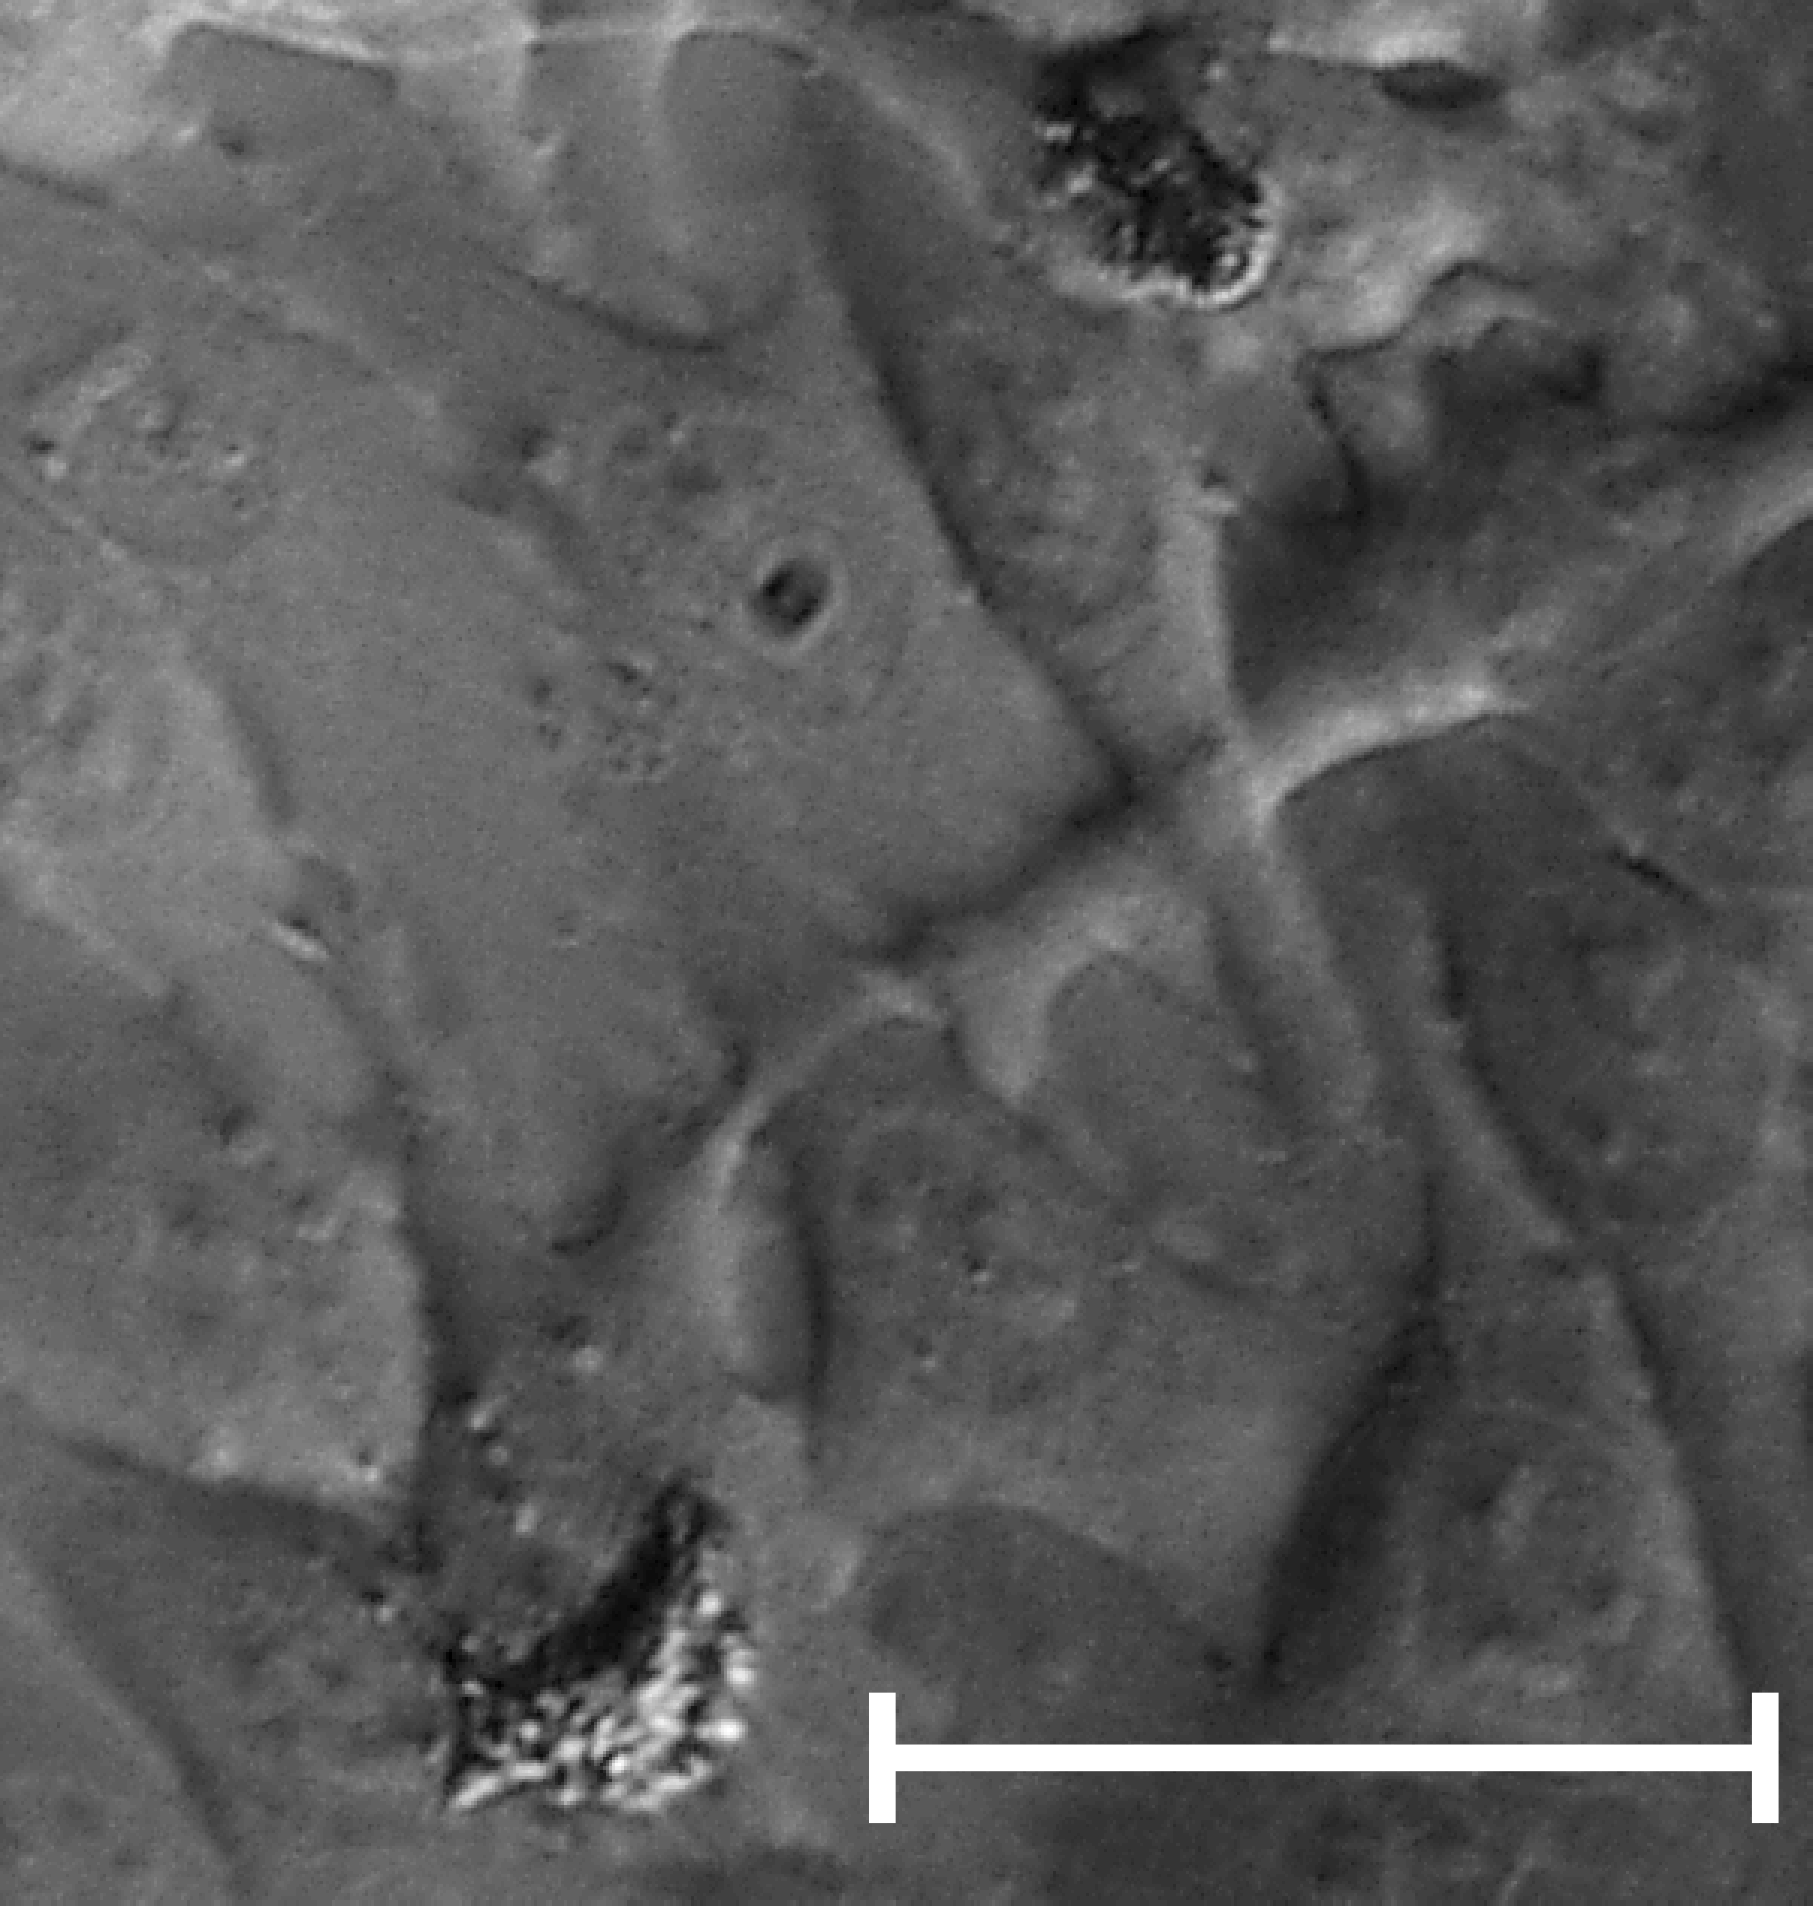
\includegraphics[width=0.45\textwidth]{Figures/Supplementary/05_White_Light/white_light_scale.png}
	\caption{White light transmission image of the sample with cells deposited on
	top of the rods. It is possible to observe that they cover entirely the
	observed region without spacing in between them. The scale bar in the figure
	is $20\um$ in length.}
	\label{fig:white-light}
\end{figure}

\section{Full scan without dye}
\begin{figure}[htp] \centering
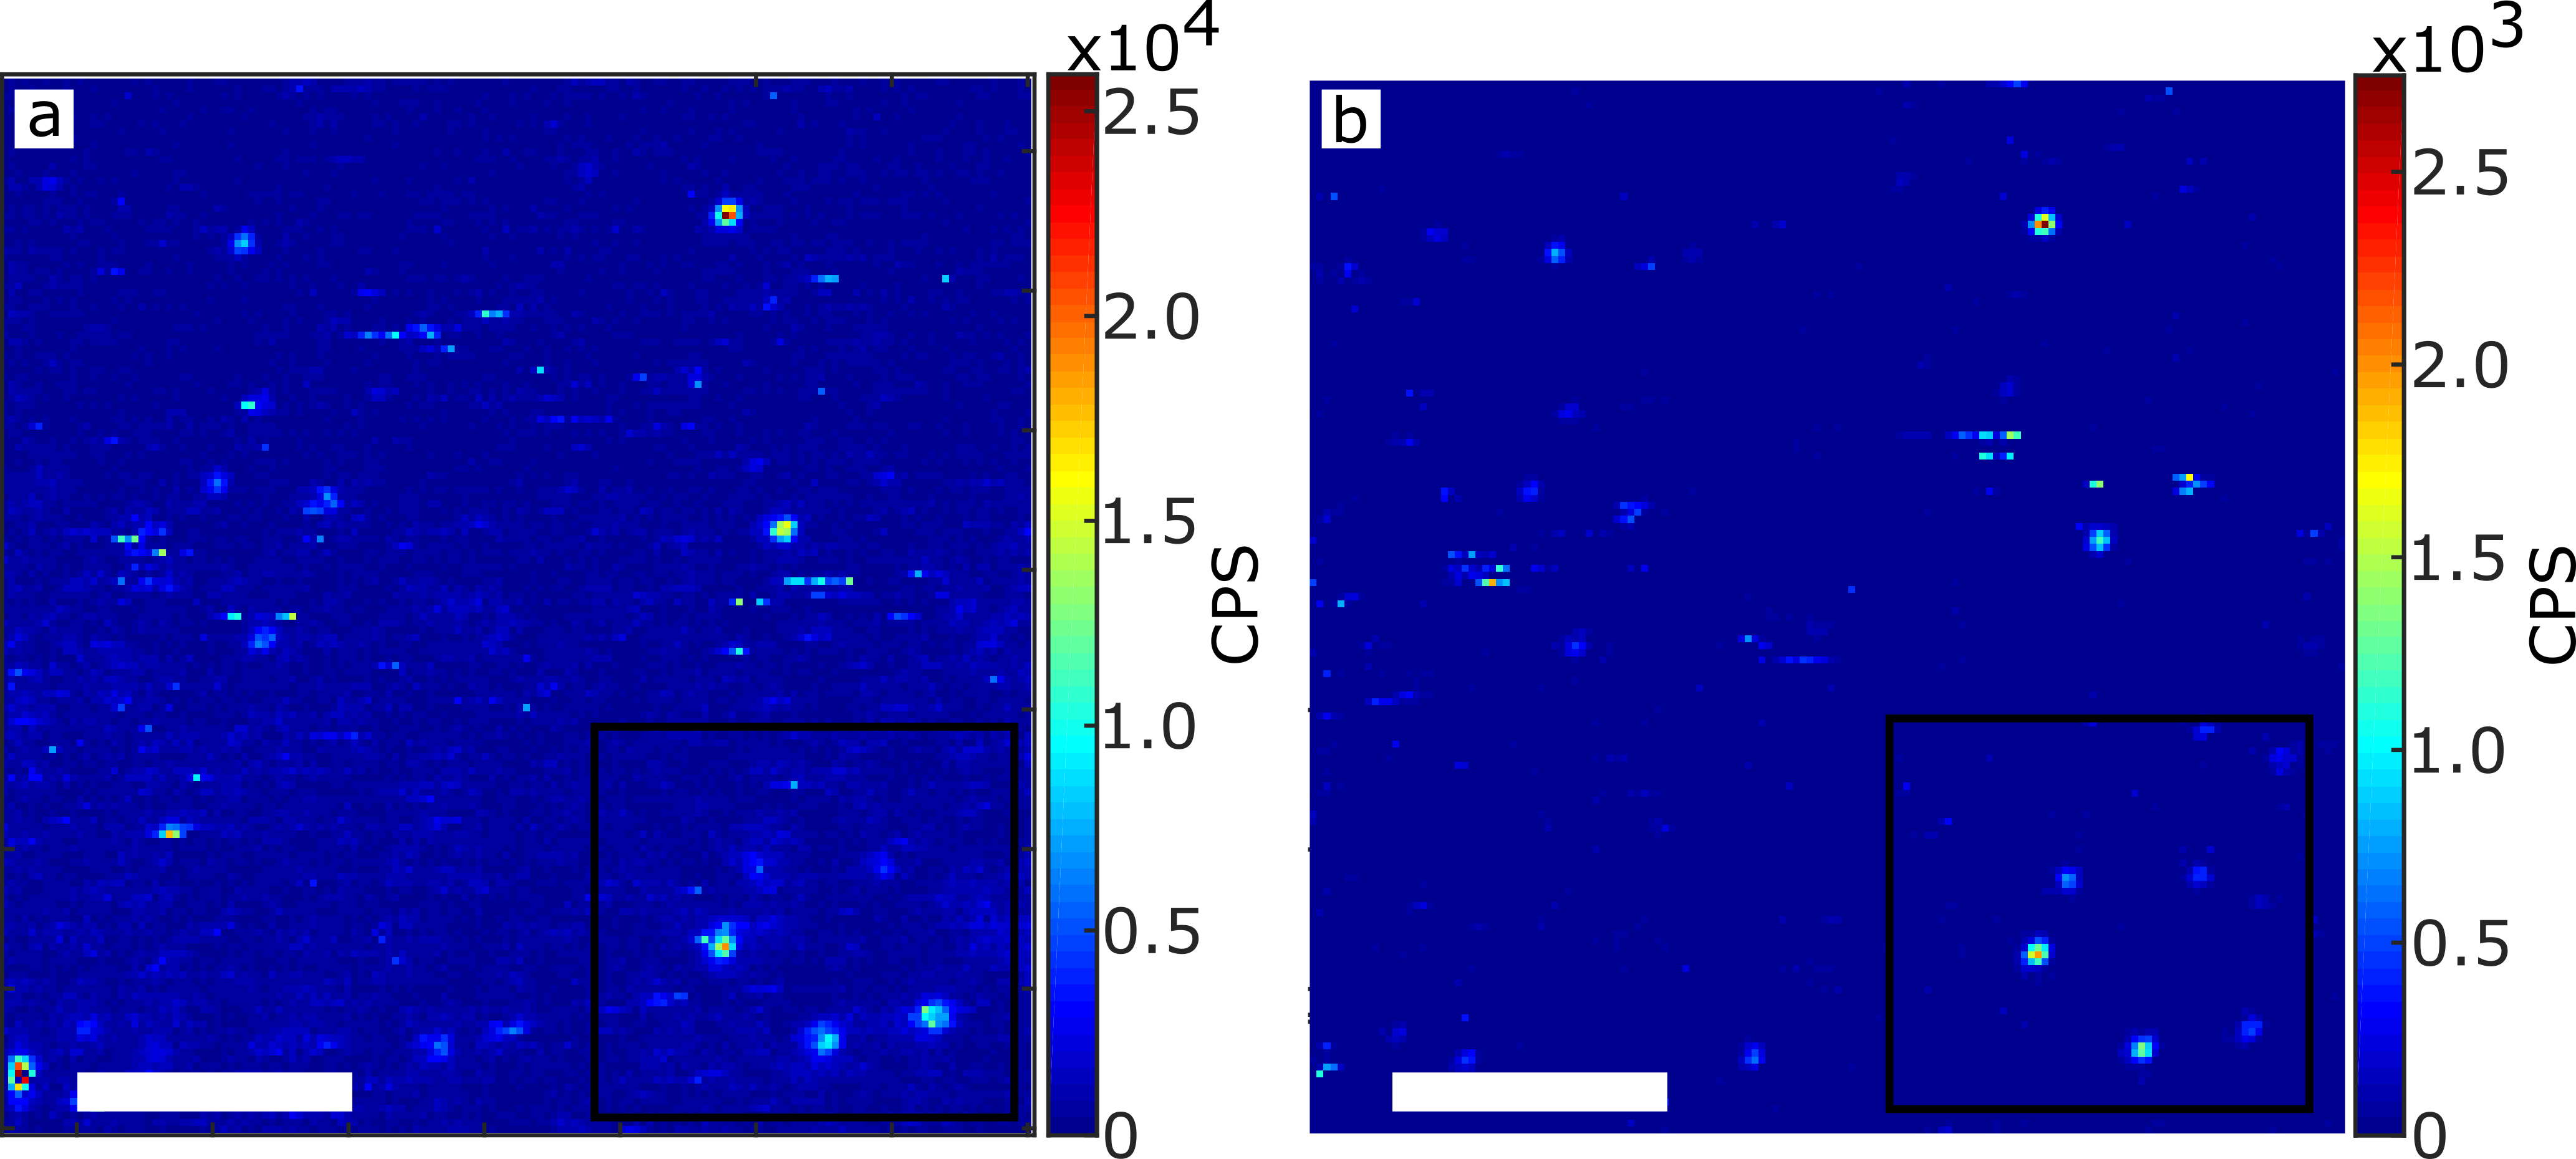
\includegraphics[width=0.95\textwidth]{Figures/Supplementary/06_Full_scans/full_no_dye.png}
\caption{Raster scan of a nanorod sample under HeLa cells using (a) a long pass
filter and (b) a short pass filter for photoluminescence detection. Both scans
contain the same region shown in the main text and here marked with a black
square. The scale bar in both figures is $4\um$ in length.}
	\label{fig:full_no_dye}
\end{figure}

The raster scan shown in Figure \ref{fig:full_no_dye} corresponds to a larger
area comprising the same region shown in the main text. The majority of the
particles has a much larger contrast in the anti-Stokes. Moreover it can be
noted that the background is flat. In the Stokes image the nanorods are still
visible, but the contrast is obviously lower.

\section{Full scan without dye}
\begin{figure}[htp] \centering
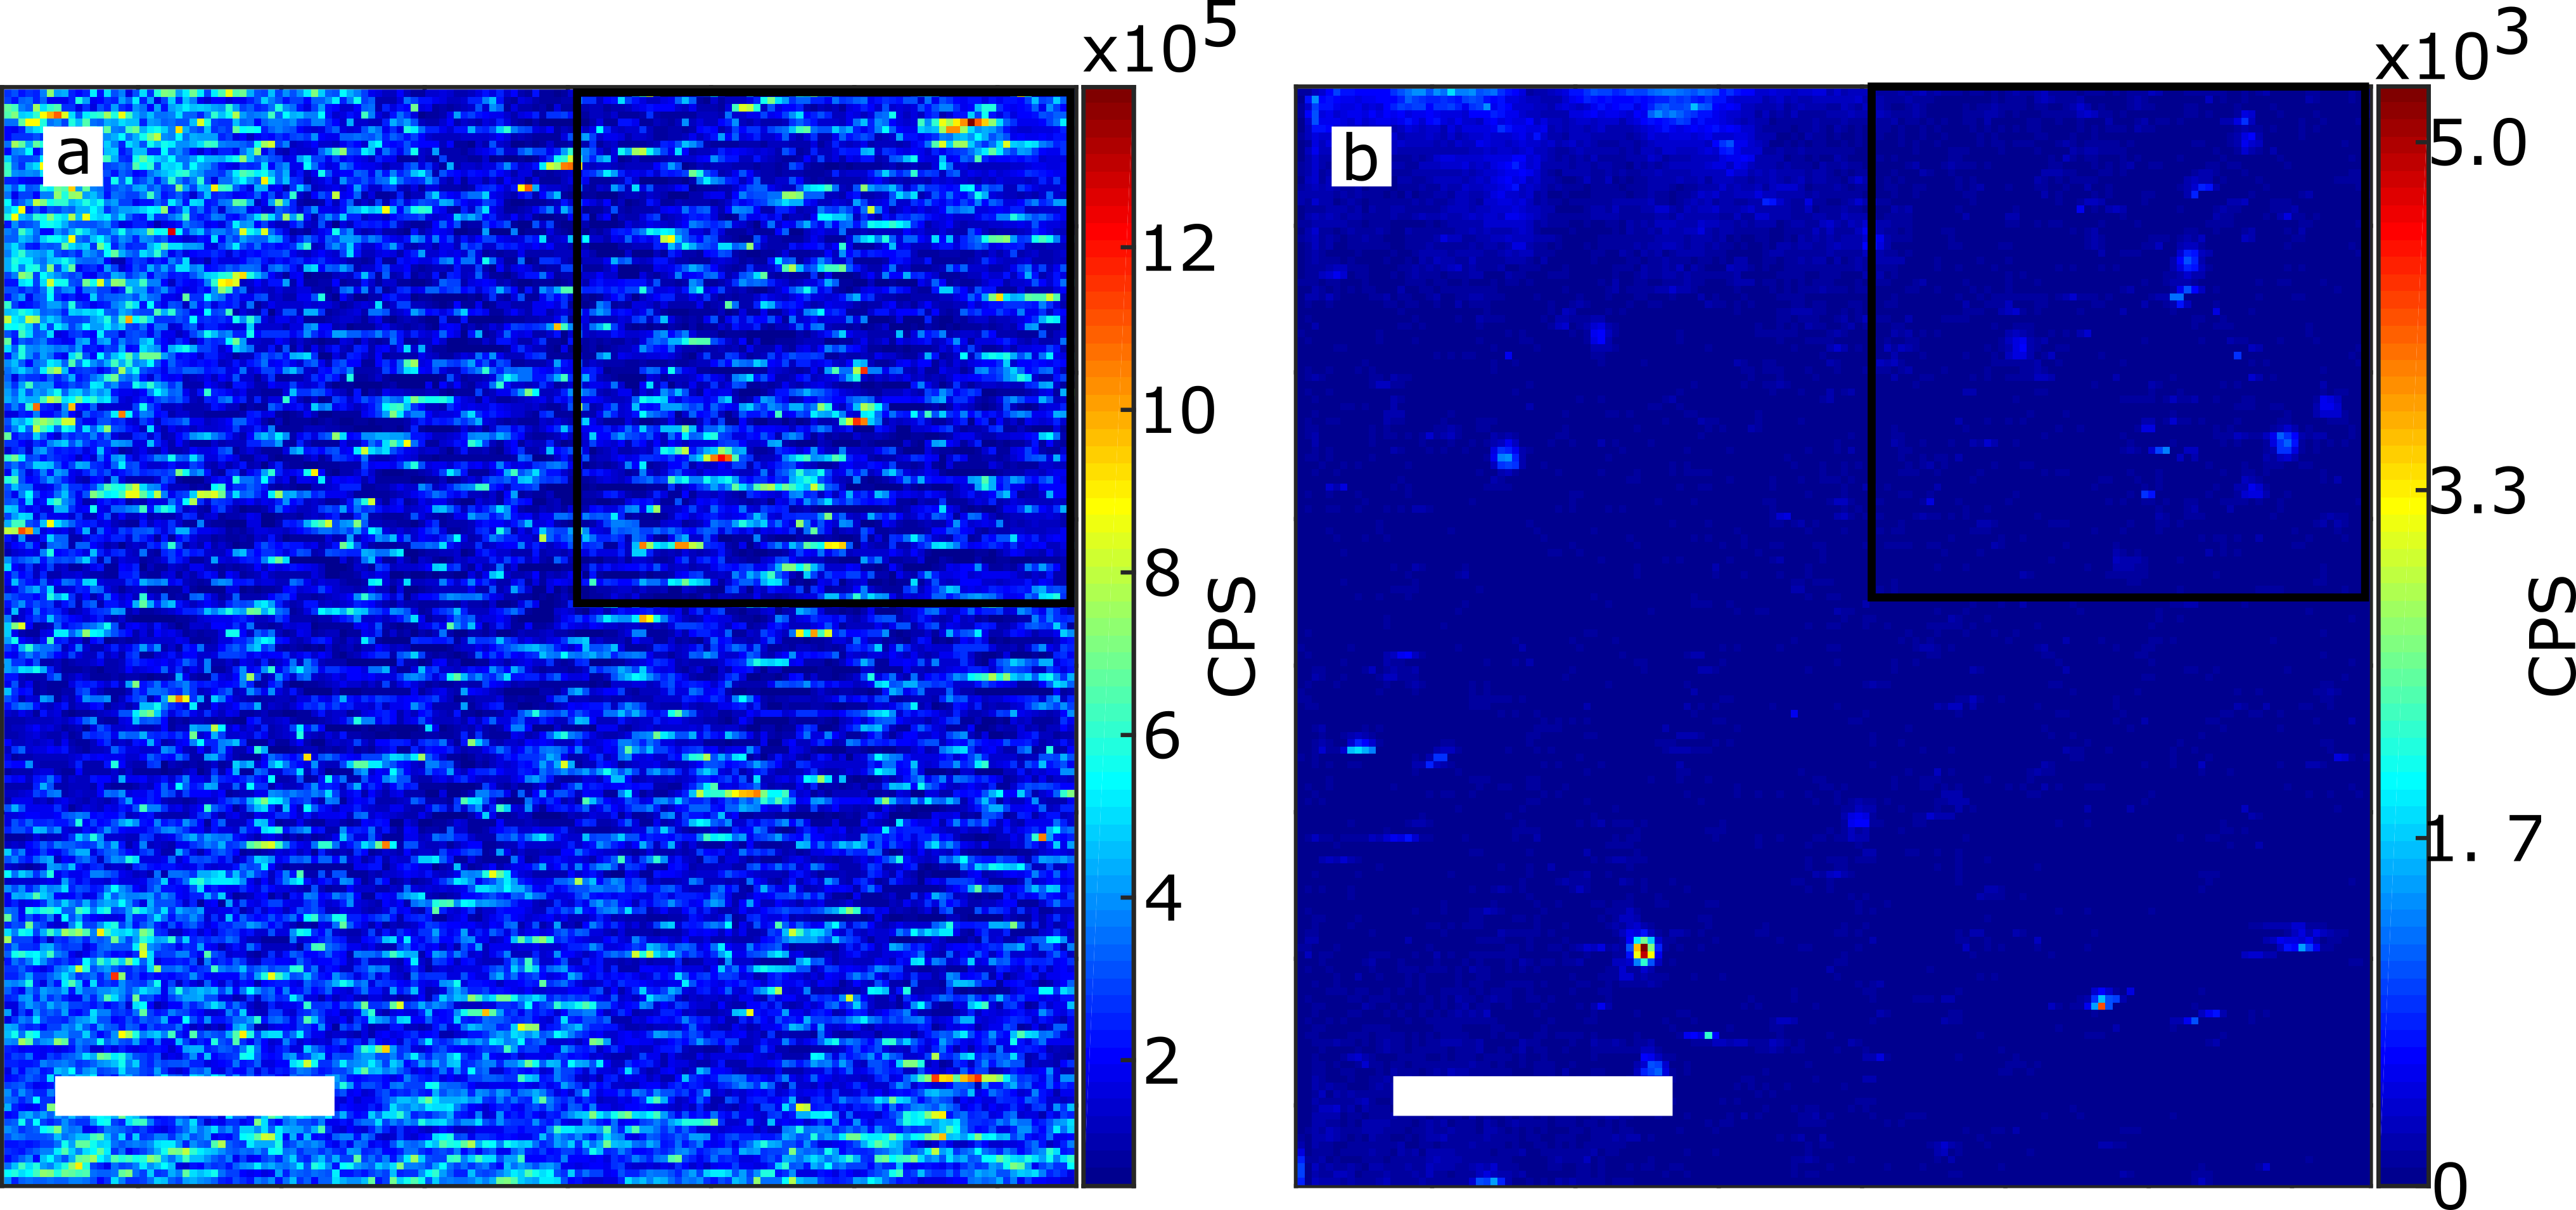
\includegraphics[width=0.95\textwidth]{Figures/Supplementary/07_Full_scans_dye/full_with_dye.png}
\caption{Raster scan of a nanorod sample under stained HeLa cells using (a) a
long pass filter and (b) a short pass filter for photoluminescence detection. Both scans
contain the same region shown in the main text and here marked with a black
square. The scale bar in both figures is $4\um$ in length.}
	\label{fig:full_with_dye}
\end{figure}

Figure \ref{fig:full_with_dye} shows a raster scan of gold nanorods under cells
stained with $\atto$. Both images comprise the same region shown in the main
text, here marked with a black square. No particles can be detected in the
Stokes image, while several nanorods are visible in the anti-Stokes image with a
high signal-to-background. We note, however, that there is some
background appearing in the top left part of the anti-Stokes image. This may be
due to an increase of the concentration of $\atto$. The incubation procedure does
not prevent the accumulation of dye in specific organelles of the cells, and
there is no control on the final dye concentration. 

\section{Signal-to-background of several particles}
\begin{figure}[htp] \centering
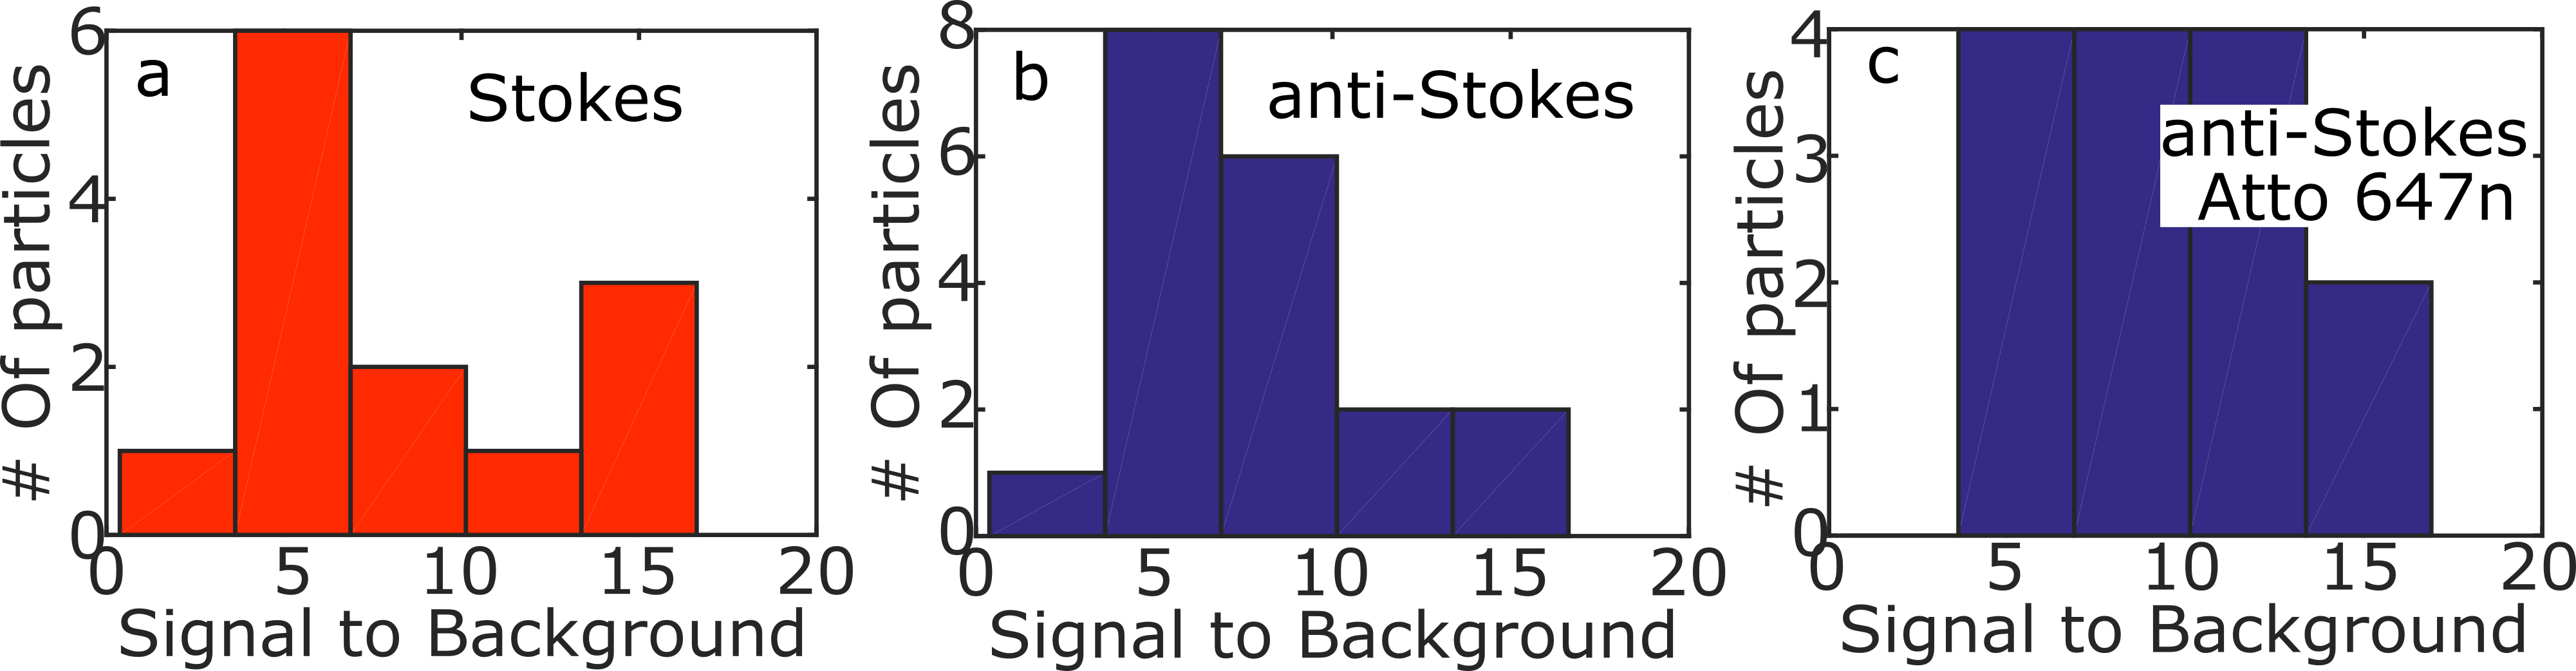
\includegraphics[width=0.95\textwidth]{Figures/Supplementary/08_Histograms_SN/08_histograms.png}
\caption{Histograms of the signal-to-background of several particles irradiated
at $30\pwr$. a) Stokes emission under unstained cells, b) same but anti-Stokes
emission, c) anti-Stokes under cells stained with \atto.}
	\label{fig:histograms_SB}
\end{figure}

Figure \ref{fig:histograms_SB} shows the distribution of signal-to-background
ratios for several particles. The data were acquired with an irradiation
intensity of $30\pwr$. Fig. \ref{fig:histograms_SB}a shows the distribution for
nanoparticles under unstained cells. It is possible to observe a broad
distribution of values between ratios of $5$ and $15$. Fig.
\ref{fig:histograms_SB}b shows the signal-to-background distribution for the
anti-Stokes emission, concentrated mainly between $5$ and $10$. Finally Figure
\ref{fig:histograms_SB}c shows the anti-Stokes signal-to-background ratio of
particles under cells stained with \atto. In this case it is possible to observe
a similar distribution of values. Stokes data under stained cells are not
presented because it was impossible to detect single nanoparticles under those
conditions. 

\section{Viability test}
\begin{figure}[htp] \centering
\includegraphics[width=0.95\textwidth]{Figures/Supplementary/09_Viability/09_viability.png}
\caption{White light transmission image of the cells, a) before being
irradiated with the $633\nm$ laser, b) after the imaging process and c)
viability test. The black square represents the imaged area. The scale bar is
$50\um$.}
	\label{fig:viability}
\end{figure}

To support the claim of the harmlessness of the method proposed in this
work, we performed a standard viability test of the cells after imaging. Figure
\ref{fig:viability} shows white light transmission images of the cells. The left
figure is before the imaging of the nanorods, the central is after and the
rightmost is the result of a viability test with trypan blue. The black square
represents the area that was imaged with the confocal microscope. The cells show
no change between before and after the procedure. Moreover in Fig.
\ref{fig:viability}c it is possible to see that the dye did not enter the cells,
therefore their membrane was intact after the imaging process. 

More rigorous tests of viability after imaging the nanorods inside the cells are
needed, but they are outside the scope of this work. On one hand there is enough
evidence showing that gold nanoparticles are not toxic for
cells\cite{Huff2007,Lewinski2008}. On the other hand two photon
imaging\cite{VandenBroek2013} or photothermal heterodyne
detection\cite{Leduc2013} of particles inside cells did not destroy them.
Continuous wave confocal imaging as presented here however was not studied in
detail in the past mainly because of the poor signal-to-background ratio with
the normal Stokes configuration.

\bibliography{BackgroundFree}

\end{document}